\documentclass[a4paper,10pt]{article}
\usepackage[utf8]{inputenc}
\usepackage{frontespizio}
\usepackage{listings}
\usepackage{pdfpages}
\usepackage[usenames,dvipsnames]{color}
\usepackage{hyperref}

\definecolor{codegreen}{rgb}{0,0.6,0}
\definecolor{codegray}{rgb}{0.5,0.5,0.5}
\definecolor{codepurple}{rgb}{0.58,0,0.82}
\definecolor{backcolour}{rgb}{0.95,0.95,0.92}

\lstdefinestyle{mystyle}{
    backgroundcolor=\color{backcolour},   
    commentstyle=\color{codegreen},
    keywordstyle=\color{magenta},
    numberstyle=\tiny\color{codegray},
    stringstyle=\color{codepurple},
    basicstyle=\footnotesize,
    breakatwhitespace=false,         
    breaklines=true,                 
    captionpos=b,                    
    keepspaces=true,                 
    numbers=left,                    
    numbersep=5pt,                  
    showspaces=false,                
    showstringspaces=false,
    showtabs=false,                  
    tabsize=2
}
\lstset{style=mystyle}

% Title Page
\title{Relazione progetto di Basi di Dati}
\author{Giovanni Liboni}


\begin{document}
\begin{frontespizio}

\Universita{Verona}
\Dipartimento{Informatica}
\Corso[Laurea]{Informatica}
\Titoletto{Consegna G4 - Sistema informativo per la gestione dell'emissione di biglietti aerei}
\Titolo{Relazione finale del progetto di Basi di Dati }

\Candidato[VR363021]{Giovanni Liboni}

\Annoaccademico{2013-2014}
\end{frontespizio}

\tableofcontents

\newpage

\part{Progetto della basi di dati}

\section{Progetto concettuale}
Qui di seguito si riporta il diagramma Entit\`a - Relazione e lo schema concettuale ricavati dalle specifiche del progetto.
A partire da questo schema si sono scritte le tabelle per la Base di Dati.

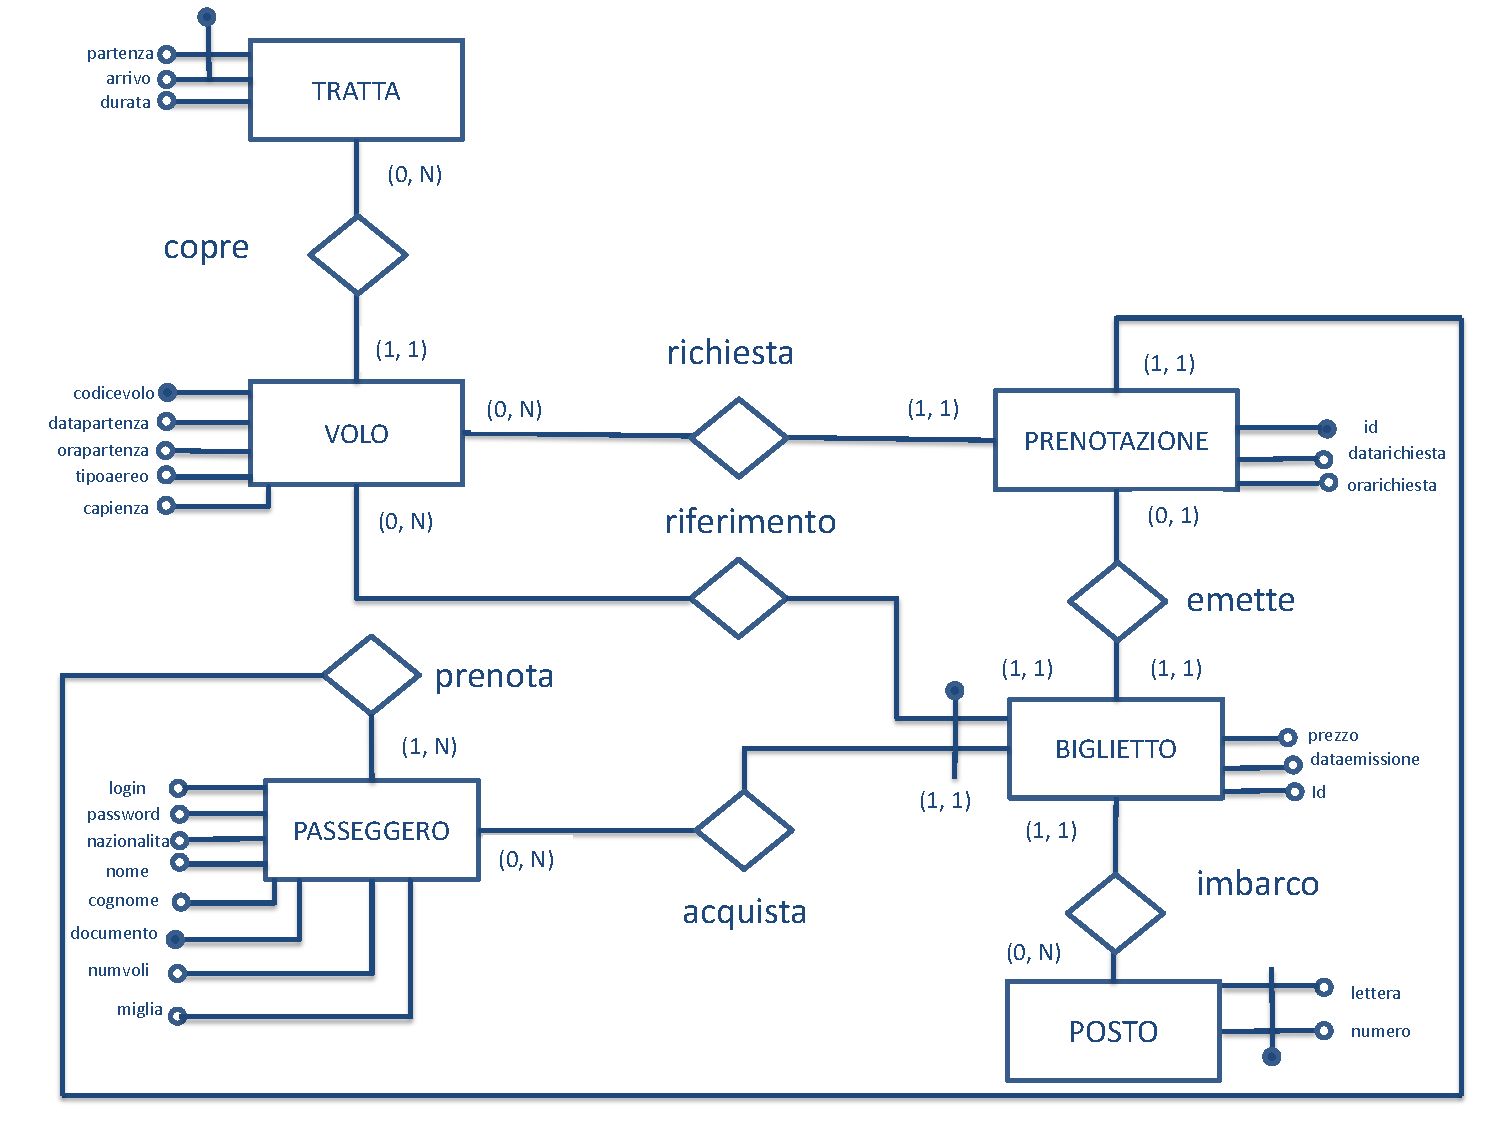
\includegraphics[scale=0.5]{er.pdf}

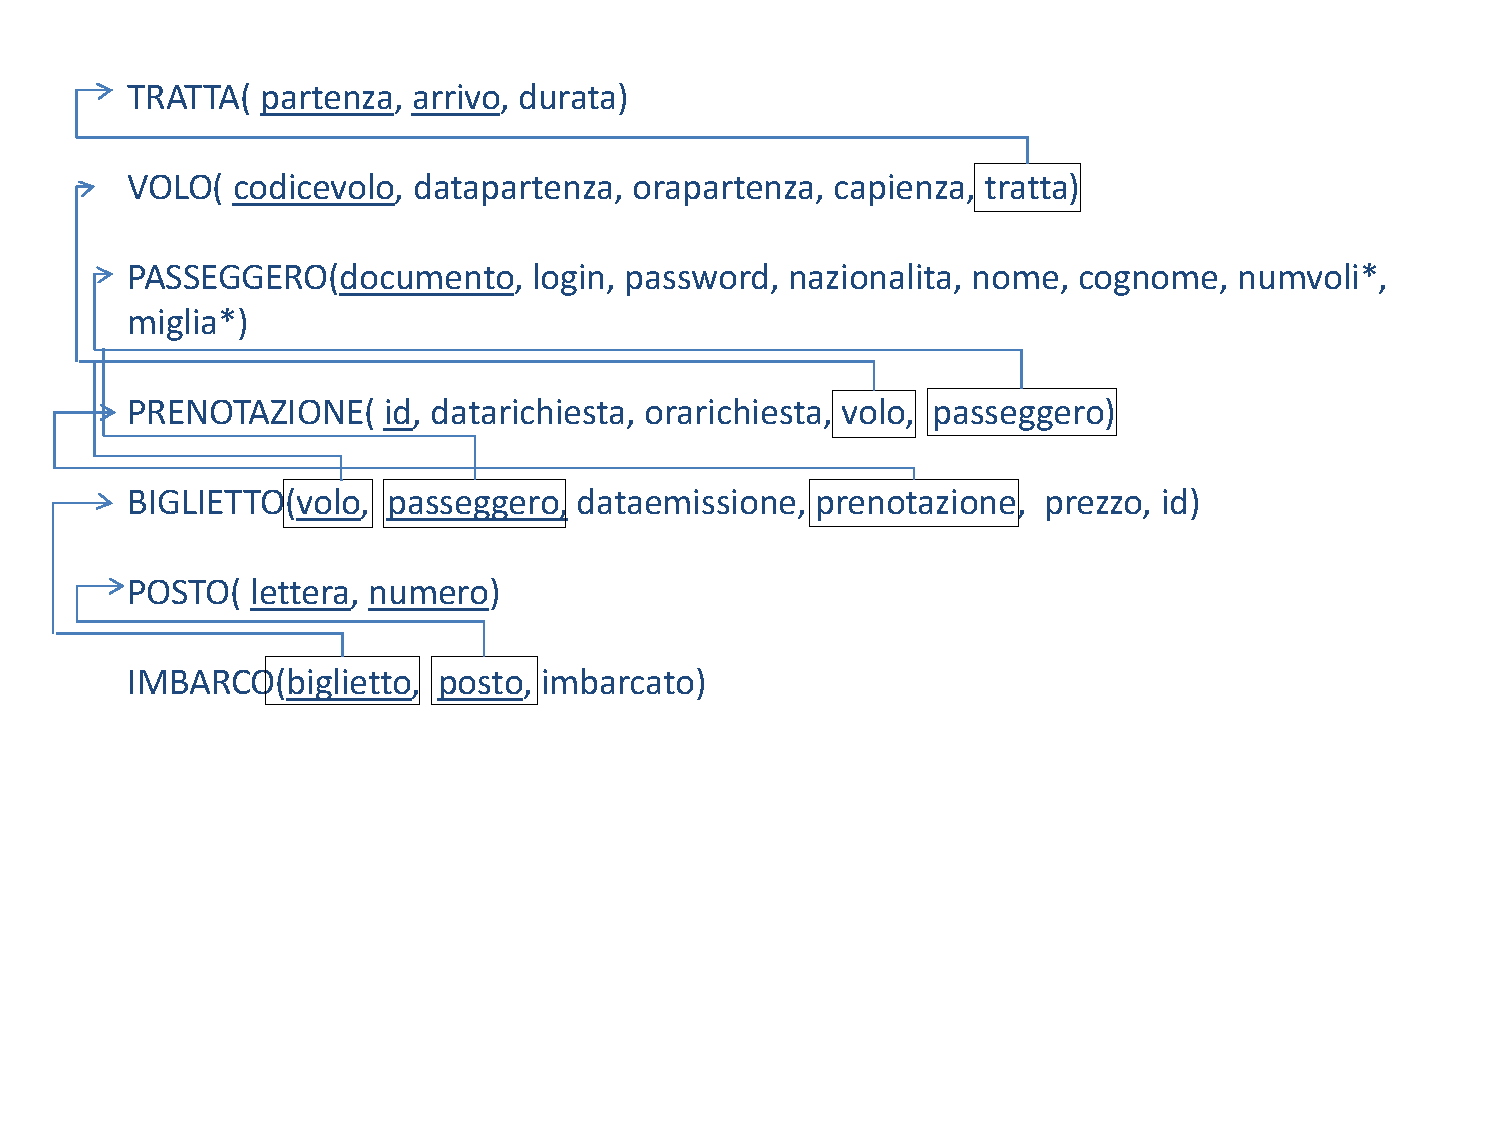
\includegraphics[scale=0.6]{schemalogico.pdf}

Descrivere il diagramma e lo schema logico.

\section{Progetto logico}

Abbiamo usato un singolo script per la creazione delle tabelle sul database. Il codice viene riportato qui di seguito.

\lstinputlisting[language=SQL, firstline=1, lastline=99]{../src/script-sql/init.sql}

Abbiamo aggiunto delle funzioni scritte in \textit{plpgsql} per eseguire azioni di routine sul base di dati e per inserire automaticamente la data e l'ora di inserimento di determinate tuple.
Si riporta di seguito il codice delle funzioni create.

\lstinputlisting[language=SQL, firstline=100, lastline=150]{../src/script-sql/init.sql}

Per automatizzare l'esecuzione delle funzioni si sono scritti dei trigger, azioni eseguite al verificarsi di certe condizioni. I trigger creati sono i seguenti:

\lstinputlisting[language=SQL, firstline=152, lastline=162]{../src/script-sql/init.sql}

\section{Popolamento della base di dati}
Per il popolamento della base di dati abbiamo creato dei programmi per la generazione automatica di query.
In particolare sono stati creati dei programmi in Java per popolare le tabelle \textit{Passeggero}, \textit{Tratta}, \textit{Volo}. I files .sql prodotti sono pronti 
per essere eseguiti senza alcuna necessit\`a di modificare il file. Le chiavi esportate vengono gestite direttamente dai programmi.


\part{Progetto del sito web}

\section{Progettazione logica}

Si riportano di seguiti gli schemi di pagina seguiti durante la creazione del sito.

\section{Struttura dell'applicazione web}

\part{Architettura MVC2}
L'elaborato \`e stato sviluppato seguendo il design pattern MVC2 e seguendo l'approccio servlet-centric. Questo pattern \`e composto da tre moduli:

\begin{itemize}
 \item MODEL -  Comprende la classe DBMS.java e i Java Data Beans. I beans sono contenuti nel package \textit{bean}, mentre la classe DBMS.java \`e contenuta nel 
		package \textit{database}. DBMS.java si occupa di interrogare il DB e di manipolare i dati al suo interno. 
		La comunicazione con main.java e picture.java  avviene tramite i 
		Java Data Beans in ambo le direzioni ;
 \item VIEW - Comprende tutte le JSPs, i javascript, i css e le foto profilo salvate all'interno della base di dati;
 \item CONTROLLER - Comprende le classi main.java, picture.java. Entrambe sono servlet con compiti differenti: picture.java gestisce le richieste di upload e download delle
		    immagini, main.java gestisce il resto delle rihieste GET e POST. Utilizza DBMS.java per l'iterazione con la base di dati ed inoltre 
		    gli eventuali dati alla JSP appropriata ;
\end{itemize}

\section{Model}
Fanno parte del modulo Model il DBMS e i javabeans. 
\section{View}
Fanno parte del modulo View tutte la JSPs, i javascript e i css.
\section{Controller}
Fanno parte del modulo Controller le due servlet. Le due servlet che controllano il flusso sono \textit{main.java} e \textit{picture.java}. 

La servlet \textit{picture.java} gestisce la parte multimediale dell'applicazione, caricando e scaricando dalla base di dati le foto profilo dei passeggeri.
Per ogni richiesta viene passato il parametro \textit{ps} con un determinato valore e pu\`o assumere questi valori:
\begin{itemize}
 \item uploadimage
 \item downloadimage
\end{itemize}

La servlet \textit{main.java} controlla le richieste da parte delle JSPs.

\begin{itemize}
 \item \textbf{areapersonale} - Vengono caricati dalla base di dati i voli e le prenotazioni dell'utente specificato nel parametro \textit{pass}. Viene passato il controllo 
			a \textit{areapersonale.jsp}. Non sono richiesti ulteriori parametri in quanto i dati del passeggero vengono recuperati dall'attributo di sessione
			\textit{pass}.

 \item \textbf{ricercavolo} - Vengono caricati gli aeroporti di partenza e viene passato il controllo a \textit{ricercavolo.jsp}.
 \item \textbf{volipage} - Ricerca un volo a partire dai valori specificati nei parametri passati e passa il controllo a \textit{voliPage.jsp} se esiste almeno una corrispondeza, altrimenti
		  viene passato il controllo a \textit{ricercavolo.jsp}.
		  I parametri richiesti sono:
		  \begin{itemize}
		   \item \textbf{partenza} Aeroporto di partenza
		   \item \textbf{arrivo} Aeroporto di arrivo
		   \item \textbf{date} Data di partenza del volo
		  \end{itemize}

 \item \textbf{prenotazione} - Recupera le informazioni del volo e del passeggero. Infine passa il controllo a \textit{prenotazionePage.jsp}. 
				I parametri richiesti sono:
				\begin{itemize}
				 \item \textbf{codiceVolo} Codice del volo per recuperare le informazioni
				\end{itemize}
				
				Non serve specificare un parametro per il passeggero in quanto le informazioni vengo recuperate dall'attributo della sessione.

 \item \textbf{nuovaprenotazione} - Vengono inviati i dati dalla form \textit{prenotazione} di \textit{prenotazionePage.jsp}, se i dati sono validi allora si procede 
				     ad aggiungere una nuova prenotazione del database. Se il passeggero non esiste ed \`e la prima volta che effettua una prenotazione
				     allora sar\`a creato un nuovo passeggero a partire dai dati passati alla servlet. Il controllo poi passa a \textit{esitoPage.jsp} con 
				     il relativo messaggio di stato.
				     I parametri richiesti sono:
				     \begin{itemize}
				      \item \textbf{nome} Nome del passeggero
				      \item \textbf{cognome} Cognome del passeggero
				      \item \textbf{documento} Numero del documento, pu\`o essere sia il numero di una carta d'identit\`a sia di un passaporto
				      \item \textbf{nazionalita} Nazionalit\`a del passeggero
				      \item \textbf{username} Username scelto dal passeggero
				      \item \textbf{password} Password scelta dal passeggero
				      \item \textbf{codicevolo} Codice del volo da prenotare
				      \item \textbf{tessera} Richiesta della tessera
				     \end{itemize}

 \item \textbf{logout} - Viene rimosso il passeggero loggato e passa il controllo a \textit{ricercavolo.jsp} insieme agli aeroporti di partenza.
 \item \textbf{login} - Vengono ricevuti la coppia login e password dalla form \textit{authentication} di \textit{login.jsp}. Se la coppia \`e valida allora passa il controllo
			 a \textit{bigliettiPage.jsp} insieme ai dati del passeggero, delle prenotazioni e dei voli. Altrimenti imposta un messaggio di errore e passa il controllo
			 a \textit{login.jsp}
			 I parametri richiesti sono:
			 \begin{itemize}
			  \item \textbf{username} Username del passeggero
			  \item \textbf{password} Password del passeggero
			 \end{itemize}

 \item \textbf{contatti} - Viene passato il controllo a \textit{contatti.jsp}
 \item \textbf{emettibiglietto} - Passa il numero della prenotazionen a \textit{emettiBigliettoPage.jsp} e gli passa il controllo. 
				  I parametri richiesti sono:
				   \begin{itemize}
				    \item \textbf{numPrenotazione} Numero della prenotazione per la quale emettere il biglietto
				   \end{itemize}

 \item \textbf{newbiglietto} - Viene richiesto di emettere un biglietto a partire dal numero della prenotazione. Una volta inserito il biglietto passa il controllo a 
 \item \textbf{chisiamo} 
 \item \textbf{ajaxricercavolo}
 \item \textbf{checkusername}
 \item \textbf{checkdocumento}
\end{itemize}

\section{Path e Context}
Il context del sito web \`e \textit{basi}, mentre il path relativo per raggiungere la servlet \`e \textit{servlet/main}. La porta del server \`e la \textit{8080}.
Quindi l'url per accedere al sito web \`e: \url{http://localhost:8080/basi/servlet/main}


\part{Scelte progettuali}

\section{Hibernate}
\section{AJAX}
\section{Session}

\end{document}          
